\documentclass{standalone}

\usepackage{tikz}
\usepackage{amssymb}
\usetikzlibrary{calc, positioning, shapes.geometric, decorations.markings}
\begin{document}
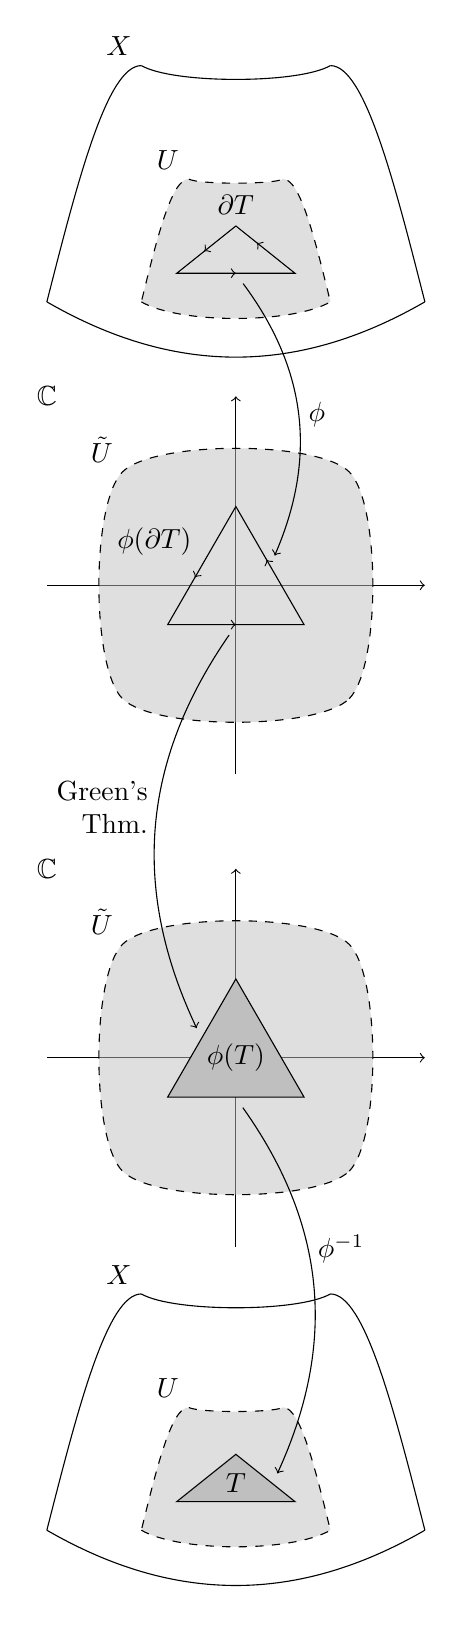
\begin{tikzpicture}[scale=1.2]
	\begin{scope}
		\coordinate (a) at (-2,-2);
		\coordinate (b) at (2,-2);
		\coordinate[label=above left:{$ X $}] (c) at (-1,0.5);
		\coordinate (d) at (1,0.5);
		\draw[bend right] (a) to (b);
		\draw[bend right, looseness=0.5] (c) to (d);
		\draw (b) sin (d);
		\draw (a) sin (c);

		\coordinate (t) at (0,-1.5);
		\coordinate (Ua) at ($ (t) + (-1,-0.5) $);
		\coordinate (Ub) at ($ (t) + (1, -0.5) $);
		\coordinate[label=above left:{$ U $}] (Uc) at ($ (t) + (-0.5, 0.8) $);
		\coordinate (Ud) at ($ (t) + (0.5, 0.8) $);

		\filldraw[dashed, fill=gray!50, fill opacity=0.5] (Ua) to[bend right, looseness=0.6] (Ub) sin
		(Ud) to[bend left, looseness=0.3] (Uc) cos cycle;

		\begin{scope}[decoration = {
						markings,
						mark=at position .15 with {\arrow{>}},
						mark=at position .5 with {\arrow{>}},
						mark=at position .9 with {\arrow{>}},
					}]
			\node[isosceles triangle, isosceles triangle stretches, shape border
				rotate=90, minimum width=1.5cm, minimum height=0.6cm, draw, label={above:$
							\partial T $}, postaction=decorate] (T) at (t) {};
		\end{scope}
		\node (l1) at (T.south){};
	\end{scope}

	\begin{scope}[yshift=-5cm]
		\draw[->] (-2,0) to (2,0);
		\draw[->] (0,-2) to (0,2);
		\node at (-2,2){$ \mathbb{C} $};

		\draw[dashed, fill=gray!50, fill opacity=0.5] plot[smooth cycle] coordinates
			{(-1.2,-1.2) (1.2,-1.2) (1.2,1.2) (-1.2,1.2)};
		\node[above left] at (-1.2,1.2) {$ \tilde{U} $};
		\begin{scope}[decoration = {
						markings,
						mark=at position .2 with {\arrow{>}},
						mark=at position .5 with {\arrow{>}},
						mark=at position .85 with {\arrow{>}},
					}]
			\node[regular polygon, regular polygon sides=3, minimum size=2cm,
				label={side 1:$ \phi(\partial T) $}, draw, postaction=decorate] (fT) at (0,0) {};
		\end{scope}
		\node (l2) at (fT.side 3){};
		\node (l2') at (fT.side 2){};
	\end{scope}

	\begin{scope}[yshift=-10cm]
		\draw[->] (-2,0) to (2,0);
		\draw[->] (0,-2) to (0,2);
		\node at (-2,2){$ \mathbb{C} $};

		\draw[dashed, fill=gray!50, fill opacity=0.5] plot[smooth cycle] coordinates
			{(-1.2,-1.2) (1.2,-1.2) (1.2,1.2) (-1.2,1.2)};
		\node[above left] at (-1.2,1.2) {$ \tilde{U} $};
		\node[regular polygon, regular polygon sides=3, minimum size=2cm,
			label={center:$ \phi(T) $}, draw, fill=gray!50] (fT2) at (0,0) {};
		\node (l3) at (fT2.side 1){};
		\node (l3') at (fT2.side 2){};
	\end{scope}

	\begin{scope}[yshift=-13cm]
		\coordinate (a) at (-2,-2);
		\coordinate (b) at (2,-2);
		\coordinate[label=above left:{$ X $}] (c) at (-1,0.5);
		\coordinate (d) at (1,0.5);
		\draw[bend right] (a) to (b);
		\draw[bend right, looseness=0.5] (c) to (d);
		\draw (b) sin (d);
		\draw (a) sin (c);

		\coordinate (t) at (0,-1.5);
		\coordinate (Ua) at ($ (t) + (-1,-0.5) $);
		\coordinate (Ub) at ($ (t) + (1, -0.5) $);
		\coordinate[label=above left:{$ U $}] (Uc) at ($ (t) + (-0.5, 0.8) $);
		\coordinate (Ud) at ($ (t) + (0.5, 0.8) $);

		\filldraw[dashed, fill=gray!50, fill opacity=0.5] (Ua) to[bend right, looseness=0.6] (Ub) sin
		(Ud) to[bend left, looseness=0.3] (Uc) cos cycle;

		\node[isosceles triangle, isosceles triangle stretches, shape border
			rotate=90, minimum width=1.5cm, minimum height=0.6cm, draw, label={center:$
						T $}, fill=gray!50] (T2) at (t) {};
		\node (l4) at (T2.east){};
	\end{scope}

	\draw[->, bend left] (l1) to node[right]{$ \phi $} (l2);
	\draw[->, bend right] (l2') to node[left, align=right, pos=0.45]{Green's\\ Thm.} (l3);
	\draw[->, bend left] (l3') to node[right, pos=0.4]{$ \phi ^{-1} $} (l4);

\end{tikzpicture}
\end{document}
